\chapter{Background}

\section{History of machine translation}

\XXX{is it ok to quote the whole paragraph with short history? e.g. \cite{Han2016}}

\section{Transformer model}

Introduced in \perscite{vaswani-2017-transformer} Transformer model is used as a base
for numerous state-of-the-art systems as can be seen for example in 
WMT18 \parcite{bojar-etal-2018-findings} and
WMT19 \parcite{barrault-EtAl:2019:WMT} results.

Prior to invention of the \textit{Transformer} model, RNN's and CNN's were used
to encode source side of the sentence pair and to decode it into the target sentence.
Various window lengths in CNN architectures allowed to capture long range relations
as well as short range ones; still the range was limited by the maximum window length.
In RNN-like architectures LSTM and GRU cells were used, as their structure allowed to
pass the internal state on longer distances due to selective forgetting.

\textit{Transformer} model uses \textit{self attention} mechanism to encode contextual
information in each word position. \textit{Position encoding} allows passing the position
information without explisit sequential connections as in RNNs.
As was stated by \textit{Transformer}'s authors, there are three main points why
self-attention mechanism should be preferred:
\begin{itemize}
  \item total computational complexity per layer;
  \item the amount of computation that can be parallelized;
  \item the path length between long-range dependencies in the network.
\end{itemize}

\begin{table}
\centering
\begin{tabular}{l|ccc}
\toprule
Layer type        &   Complexity             &  Sequential & Maximum        \\
                  &   per layer              &  operations & path length    \\
\midrule
Self-Attention    & $O(n^2 \cdot d)$         & $O(1)$      & $O(1)$         \\
Recurrent         & $O(n \cdot d^2)$         & $O(n)$      & $O(n)$         \\
Convolutional     & $O(k \cdot n \cdot d^2)$ & $O(1)$      & $O(log_k (n))$ \\
Self-Attention (restricted) & $O(r \cdot n \cdot d)$       & $O(1)$ & $O(n/r)$  \\
\bottomrule
\end{tabular}
\mycaption{Maximum path lengths, per-layer complexity and minimum number of sequential operations for different layer types} {
	n is the sequence length, 
	d is the representation dimension, 
	k is the kernel size of convolutions and 
	r the size of the neighborhood in restricted self-attention.
}
\label{tab:layer_complexity_comp}
\end{table}


\begin{figure}[h]
	\centering
	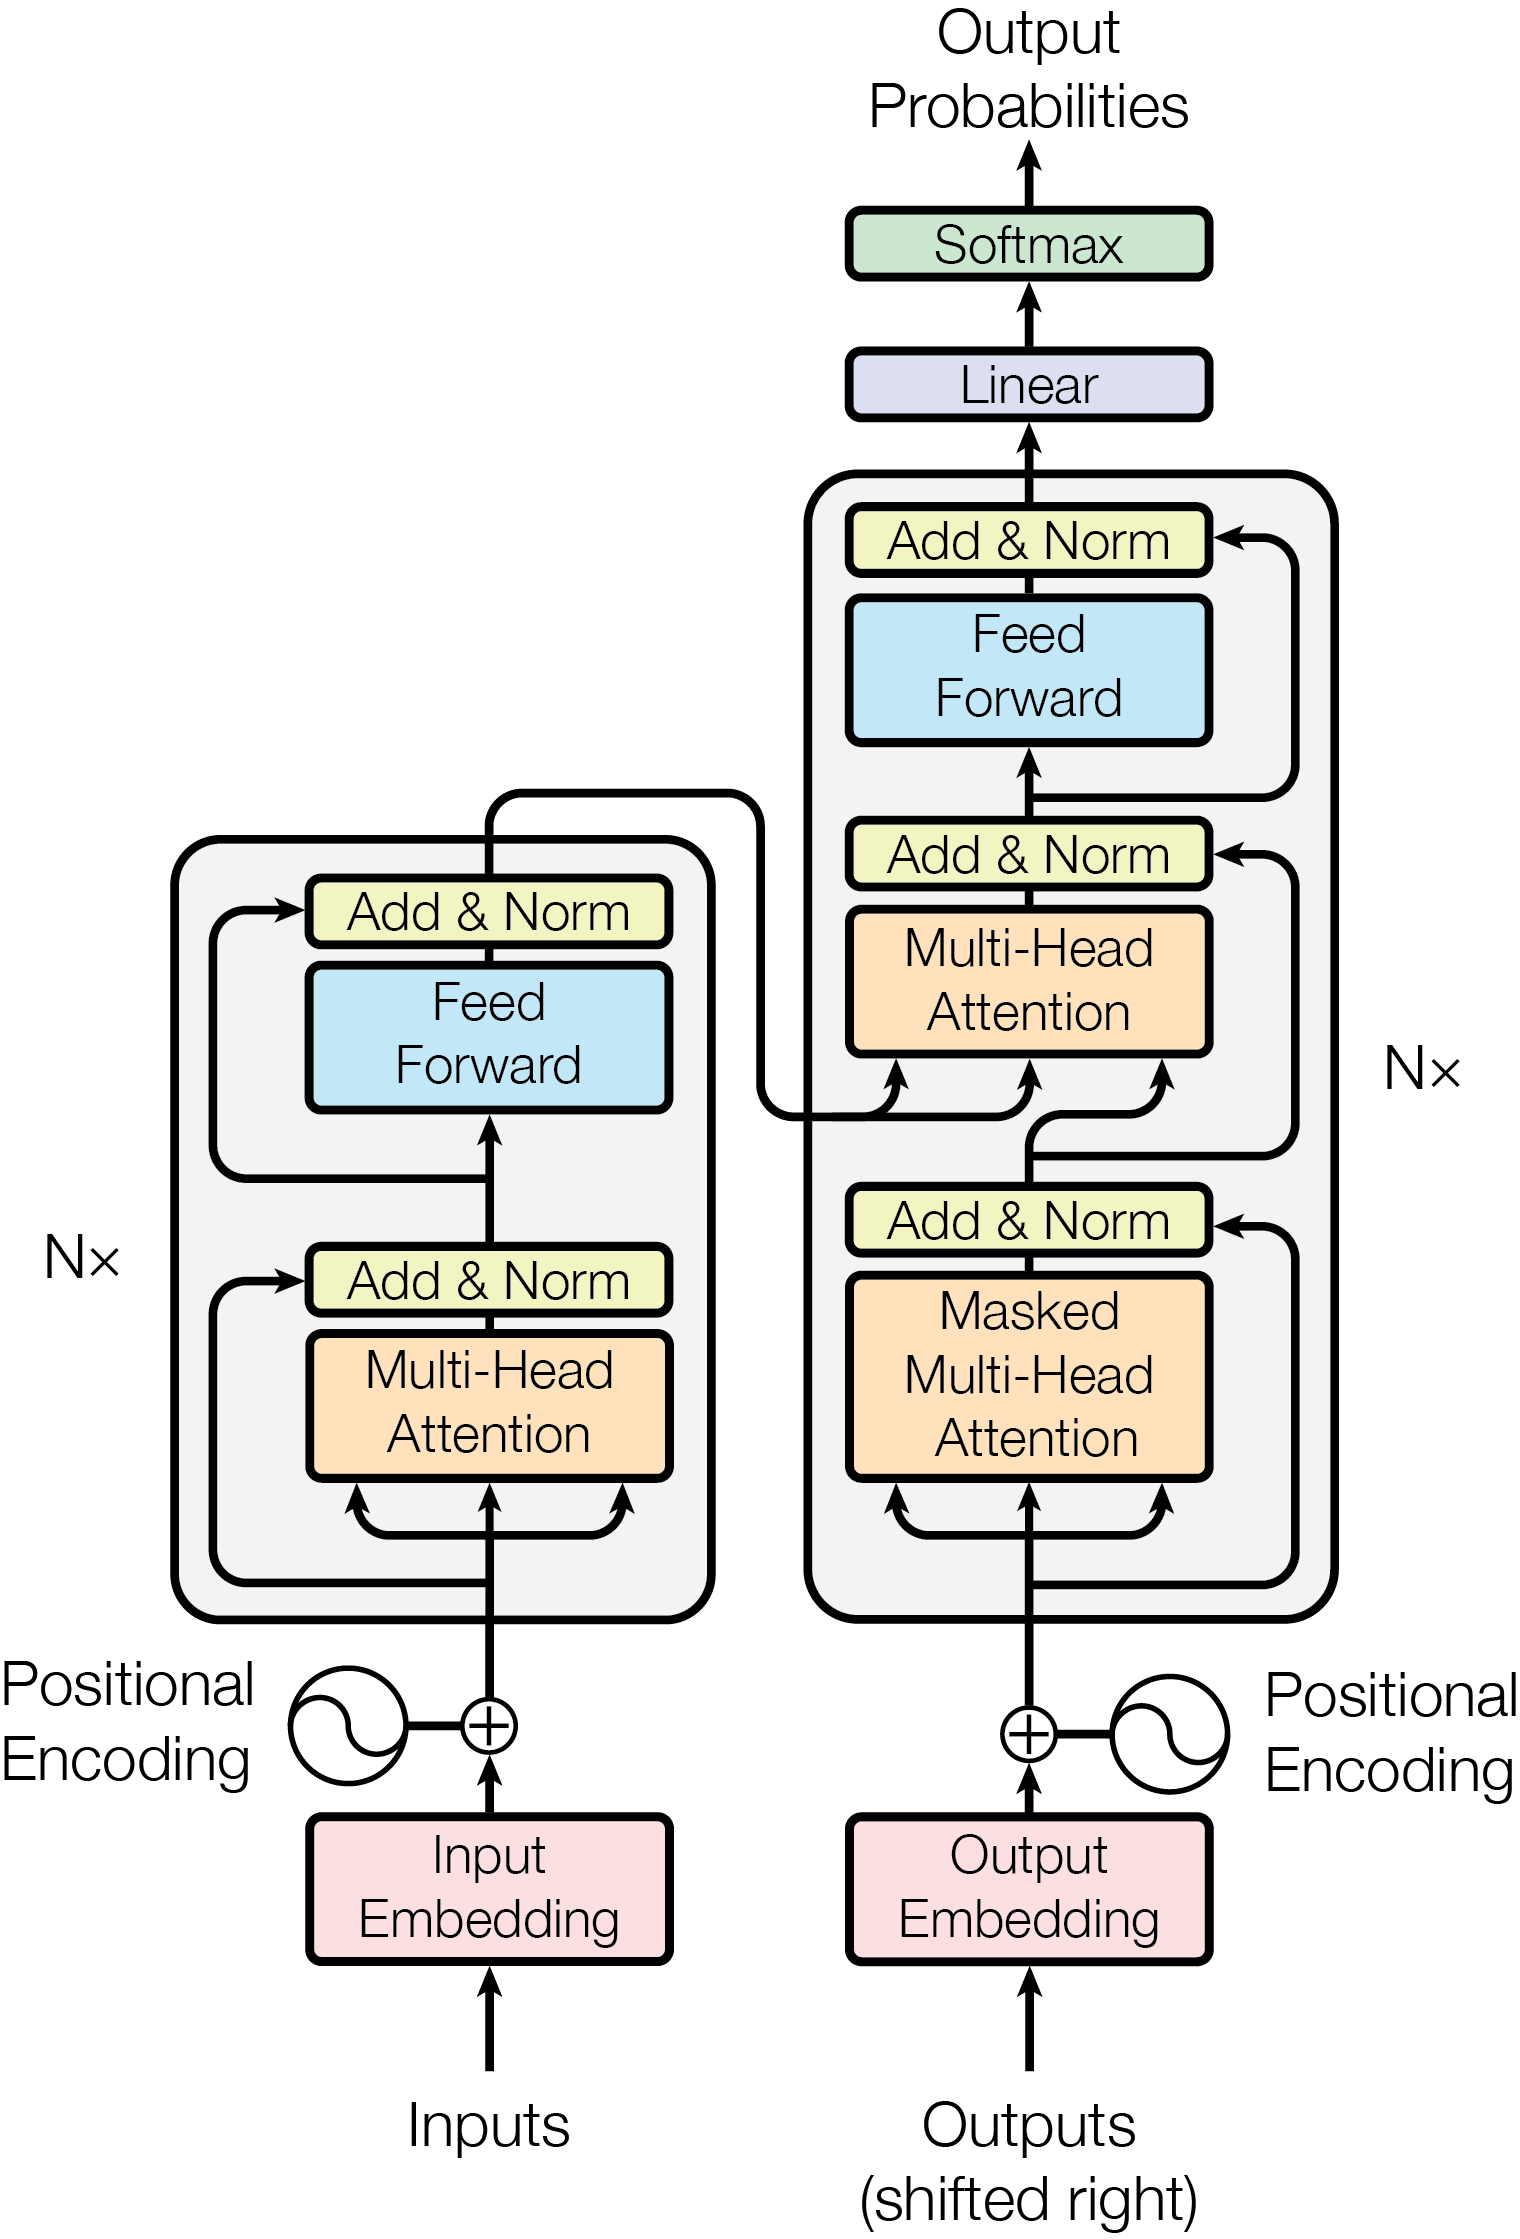
\includegraphics[width=0.9\columnwidth]{../img/transformer_architecture.png}
	\mycaption{Transformer model architecture} {}
	\label{fig:transformer_architecture}
\end{figure}

\section{Translation evaluation}

\subsection*{History}

In 1966 first machine translation evaluation methods were proposed
by the automatic language processing advisory committee (ALPAC).
The proposed metrics were "intelligibility" and "fidelity"\citep[p~67]{Translation1966}.
Metrics were considered independent and the evaluation was meant to be conducted
by two independent groups of raters.
\textit{Intelligibility} was measured without reference to the original by
group of raters fluent in target language and not familiar with the source language.
The raters were comparing the "informativeness" of evaluated translation with carefully
prepared reference translation. The metric scale was from 1 (hopelessly unintelligible)
to 9 (perfectly clear and intelligible).
\textit{Fidelity} to the sense of the original text was measured by another group of raters,
which were native speakers of the target language and highly proficient in the source language.
It was measured on a scale of 0-9 and showed how much additional information was added in
the evaluated translation comparing to the reference translation.

Advanced Research Projects Agency (ARPA)
\todo{from White 1999 and Church 1993}
comprehension evaluation, quality panel evaluation, and evaluation based on adequacy and fluency

Automatic evaluation

- Metric should correlate with human judgments;

- Works with texts of different domains

- Banerjee et al. (2005) correlation, sensitivity, consistency, reliability and generality.

\subsection*{BLEU - bilingual evaluation understudy}

In \cite{Papineni02bleu} was introduced a nowel method of audomatic machine translation evaluation -
BLEU (bilingual evaluation understudy). Its advantages are high speed and low cost of evaluation,
language independence and high correlation with judgements of highly skilled human raters evaluations.

Shortly, BLEU score incorporates modified n-gram precision scores corrected by brevity penalty,
which ensures the produced translation lenght is close to the reference one.
BLEU score is computed for the whole test corpus.

\subsubsection*{Modified \textit{n}-gram precision score}

The main element of the metric is the \textit{precision} measure.
To compute precision, the number of candidation translatin words (unigrams) that are present in
any reference translation is divided by the total number of words in the candidate translation.
This approach leads to overrating candidate translation which consist of only one or couple of
words that occur in reference translations, as can be seen in the expample below.

Intuitively, after a word from the reference translation has occured it should not be considered
in the calculation anymore. This intuition is formalized as the \textit{modified unigram precision}.
It is computed in the following way: first, the maximum number of occurances of a word in any
reference translation is counted; then the total count of every candidate word is replaced by the
maximum reference count, added up and divided by the initial total number of candidate words.
As a result, the sentence which may receive high precision score will receive more realistic evaluation
measured by modified precision score, as can be seen in the example below.\\

Candidate: \underline{of} \underline{of} \underline{of} of of of of of of of

Reference: London is the capital \underline{of} England and \underline{of} the United Kingdom
\underline{of} Great Britain and Northern Ireland.

Precision: 1

Modified unigram precision: 3/10
\\
Similarly is computed modified \textit{n}-gram precision score for any \textit{n}, but \textit{n}-gram
counts are collected instead.

\subsubsection*{Sentence length}

\subsubsection*{The formula}


\section{Multi-target machine translation}
\label{section:multitarget_mt}

\subsection{Multi-lingual machine translation}

With constant improvement of neural MT systems performance researchers started to
experiment with incorporating multiple source and/or target languages into one model,
and the results are promising: having L1\to{}L2 and L2\to{}L3 non-parallel
corpora makes possible to train a model that can produce L1\to{}L3 tranlsation
of decent quality; having high-resource L1 and low-resource L2 from the same language
group helps increase Source\to{}L2 trainslation quality with pretraining on
Source\to{}L1 data.
In general, in some situations using more target and/or source languages in one translation
model may not only unsignificantly decrease its performance but also to improve it.

Even if the concept of combining multiple languages into one model and possible outcomes
of such combination may seem intuitive, there exist multiple approaches of how exactly
this might be performed. As for current time, \cite{Dabre2019} categorizes
MNMT (multi-lingual neural machine translation) in the following way
(Figure \ref{fig:mnmt_categorized}):

\textbf{Multivay translation.}
The goal is constructing a single NMT system for one-to-many, many-to-one or many-to-many
translation using parallel corpora for more than one language pair.

\textbf{Low or Zero-Resource Translation.}
Large amount of parallel texts of high quality is available for most of European
languages. However, it is not true for most of other languages in the world.
Three main directions have been studied these cases.
\textit{Transfer learning}: Transferring translation knowledge from a high-resource language pair
to improve the translation of a low-resource language pair.
\textit{Pivot translation}: Using a high-resource language (usually English) as a pivot to translate
between a language pair.
\textit{Zero-shot translation}: Translating between language pairs without parallel corpora.

\textbf{Multi-Source Translation.} Important documents and internationally popular books have
been translated into many languages. Having the source side represented by multiple languages
may increase translation quality in general or help to remove ambiguities present in one or another
source language (e.g. cases, noun genders, etc.).


\begin{figure}[h]
	\begin{minipage}{0.9\textwidth}
	\centering
	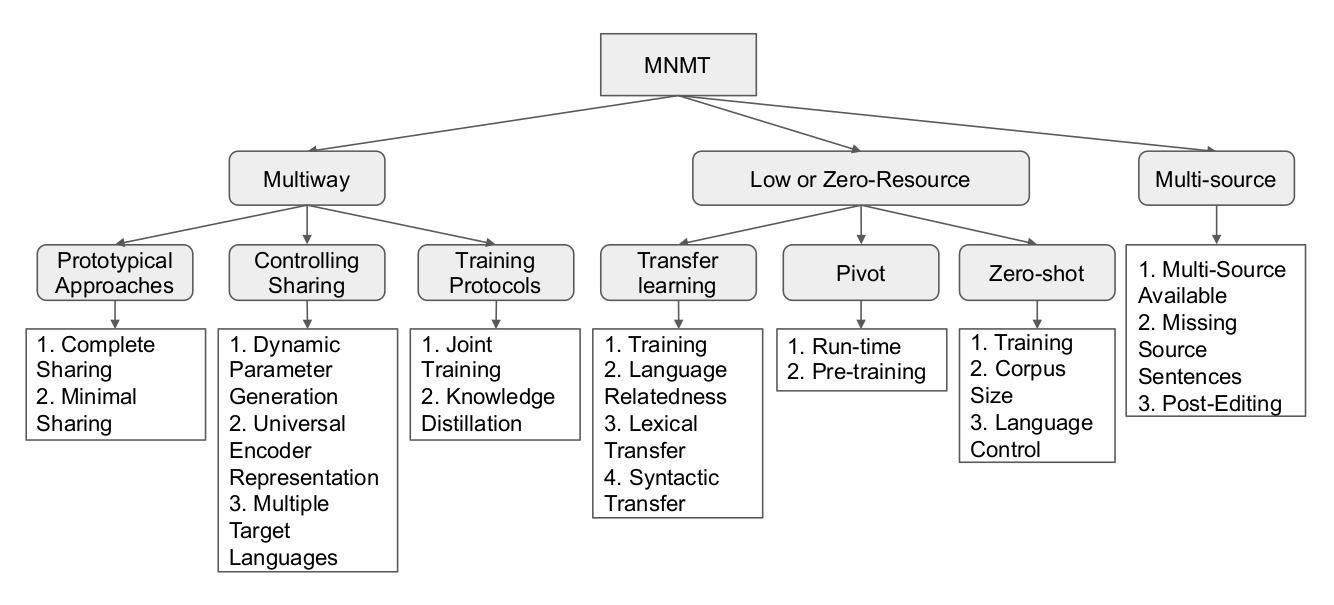
\includegraphics[width=1.0\columnwidth]{../img/dabre_2019_mnmt_categorized.png}
	\end{minipage}\hfill
	\mycaption{%
		MNMT research categorized%
	}{%
		According to resource scenarios and underlying modeling principles.
		By \cite{Dabre2019}
	}
	\label{fig:mnmt_categorized}
\end{figure}


\subsection{Massively multi-lingual machine translation with complete sharing}
\label{section:multitarget_theory}

In \cite{aharoni-etal-2019-massively} models with up to 103 languages were tested.
English centric in-house dataset was used to train En\to{}Any and Any\to{}En multilingual models.
The average number of examples per language pair is 940k:
for 13 out of the 102 pairs there were less than one million examples available.
All languages from 5-to-5 model are present in 25-to-25, same is true for all languages from 25-to-25 with respect to 50-to-50 and so forth.
In all cases they trained large Transformer model with 473.7M parameters.
As can be seen on Table \ref{tab:aharoni-2019-performance-drop}, the quality of translation
is significantly worse when model is trained to translate more languages.
However, it is worth reminding that this many-to-many experiment may have different results due to many-to-one direction present in it.

The decrease of model's performance with adding more target langueges
is clearly shown in \cite{aharoni-etal-2019-massively}.


\begin{table}[h!]
\centering
\begin{tabular}{r|cccc}
\toprule
           & En-Ar & En-Fr & En-Ru & En-Uk \\
\midrule
5-to-5     & \textbf{12.42} & \textbf{37.3} & \textbf{24.86} &         16.48  \\
25-to-25   &         11.77  &         36.79 &         23.24  & \textbf{17.17} \\
50-to-50   &         11.65  &         35.83 &         21.95  &         15.32  \\
75-to-75   &         10.69  &         34.35 &         20.7   &         14.59  \\
103-to-103 &         10.25  &         34.42 &         19.9   &         13.89  \\
\bottomrule
\end{tabular}
\mycaption{BLEU scores for translation in one direction
        (part of Table 7 from \citep{aharoni-etal-2019-massively})
	}{
		Model trained on 5-to-5 English centric dataset
		(English to any and any to English) scores 12.42 BLEU for
		English-Arabic test set. Every language from 5 languages
		of 5-to-5 data set is included into 25-to-25 set, as well
		as every language from 25-to-25 data set is included into
		50-to-50 and so forth.
	}
\label{tab:aharoni-2019-performance-drop}
\end{table}


\begin{figure}[h]
	\begin{minipage}{0.48\textwidth}
	\centering
	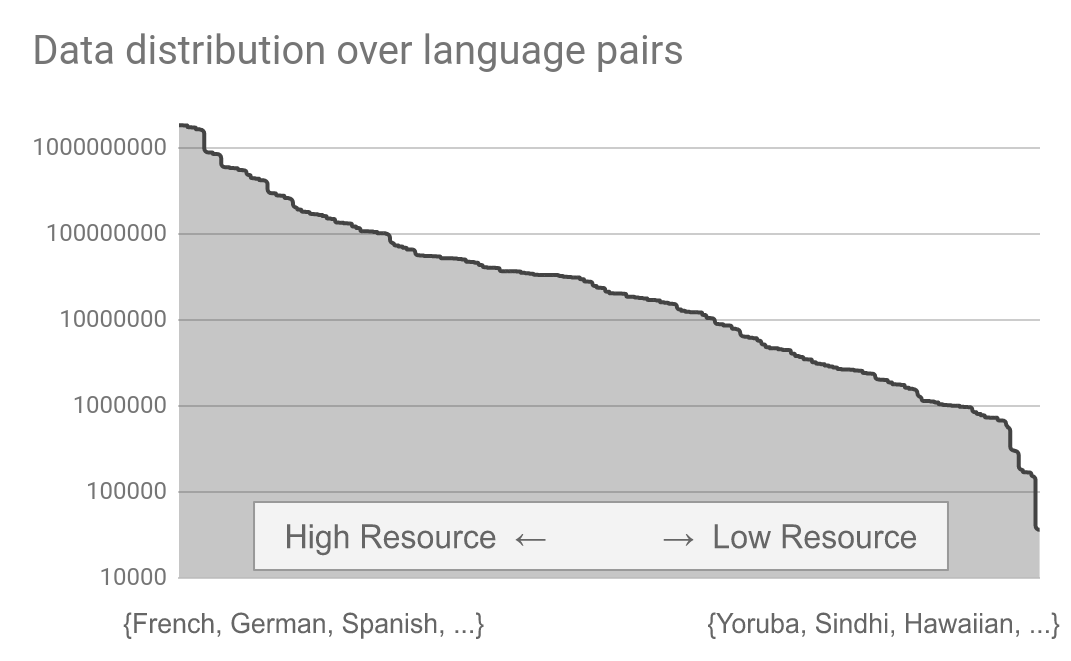
\includegraphics[width=0.9\columnwidth]{../img/arivazhagan-2019-data-distribution.png}
	\end{minipage}\hfill
	%\vspace*{\floatsep}% https://tex.stackexchange.com/q/26521/5764
	\begin{minipage}{0.48\textwidth}
	\centering
	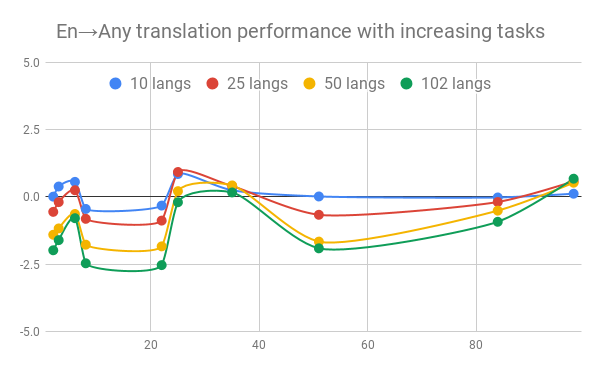
\includegraphics[width=0.9\columnwidth]{../img/arivazhagan-2019-diff-per-n-targets.png}
	\end{minipage}
	\mycaption{
		Tranlsation performance for 102 languages from
		\citet{arivazhagan-2019-mmnmt-in-the-wild}
	}{
		Axis \emph{X} is shared between left and right plot.
		On axis \emph{X} there are languages sorted by amount of training data.
		Left: amount of training data (axis \emph{Y}) for a language.
		Right (best viewed in color): Effect of increasing the number of languages on
		the translation quality. On the axis \emph{X} the languages are sorted the
		same way as on the left plot. The points visualized are 10 languages
		that are present in all setups
		from En $\leftrightarrow$ 10 to En $\leftrightarrow$ 102.
	}
	\label{fig:arivazhagan-2019-diff-per-n-targets}
\end{figure}


\subsection{Conclusion}

In this chapter we introduced theoretical and historical background for this work.
Firstly, we took a short walk through the history of machine translation.
Then we described the most used type of NMT models -- self-attention \textit{Transformer} model.
After that we went over the history of translation evaluation in general and the most
used method of automatic evaluation -- BLEU -- in particular.
In the end multi-lingual neural machine tranlsation was reviewed with more detailed view into
'complete sharing' scheme.
